\documentclass[lettersize,journal]{IEEEtran}
\usepackage[utf8]{inputenc}
\usepackage{multicol}
\usepackage{amsthm}
\usepackage{amsmath}
\newtheoremstyle{mystyle}% name
  {\topsep}% Space above
  {\topsep}% Space below
  {\normalfont}% Body font
  {}% Indent amount
  {\bfseries}% Theorem head font
  {}%Punctuation after theorem head
  {.5em}%Space after theorem head
  {}% theorem head spec
\theoremstyle{mystyle}
\newtheorem{prob}{Problem}
\usepackage{graphicx}
\usepackage{wrapfig}
 %preamble
\bibliography{finalrefs.bib}
\title{Achieving 6250fps on CMOS Active Pixel Sensor Array}
\author{LJ Gonzales*\thanks{*LJ is with the Department of Electrical and Computer Engineering, Johns Hopkins University, Baltimore, United States}}
\date{May 2022}

\begin{document}
\maketitle
\begin{abstract} We present an implementation from the ground up of a 4 by 4 APS array with readout on a shared data bus, with the TSMC 180nm process. The timing and layout design is completed with the general philosophy of repeatability and scaleability; in particular, the timing scheme is designed so as to support the addition of an arbitrary amount of rows and columns with no changes to the low-level schematic and only minor changes in timing protocol.
\end{abstract}
\section{Introduction}
Ever-increasing expertise in CMOS fabrication technology has lead to the widespread use of imaging technology for both professional use (medical and industrial equipment) and personal use. In order to meet the great demand for IoT connected devices while remaining conscious of the significant ecological impact of CMOS fabrication, designers need to ensure the longevity and flexibility of their products. To do so, we decide to take a look at the very foundations of an active pixel sensor, building up to a 2.5 by 2.5mm array (about 625 individual pixels).
\section{Global Impacts of IC Design}
Foundry services have become exceedingly affordable in the past decade: cell cost has fallen to a fraction of its original value, and cell density on a single wafer has increased accordingly. Unfortunately, Moore's law did not predict an exponential decrease in the environmental cost of IC production, and the environmental cost (primarily in water consumption, chemical waste discard, and energy consumption), remains high. TSMC alone uses "5\% [predicted to rise to 7.2\%] of all of Taiwan's electricity, [and] used about 63m tons of water in 2019" \cite{environmental}.
In today's landscape of rapidly changing technology, the modularity and flexibility of new products needs to be prioritized such as to extend their as of yet short lifespan and help alleviate the industry's pressure on global resources.
\section{Design}
\subsection{Three transistor APS}
The APS consists of 3 transistors and a photodiode (Figure \ref{apsdraw}). The photocurrent induced by incoming light discharges the source-follower gate capacitor at a rate proportional to its magnitude. Our goal is to measure this quantity, interpreted as the brightness on that pixel.
\begin{figure}[h]
	\centering
	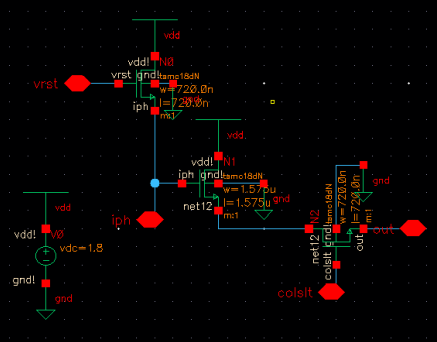
\includegraphics[width =0.3\textwidth]{apschem.png}
	\caption{3-transistor APS schematic}
	\label{apsdraw}
\end{figure}
\begin{figure}[h]
	\centering
	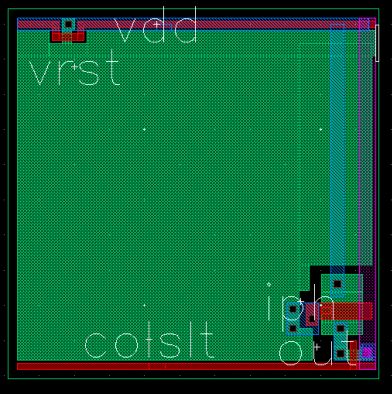
\includegraphics[width =0.3\textwidth]{apslayout.png}
	\caption{3-transistor APS layout}
	\label{apslayout}
\end{figure}

We are given that the minimum and maximum photocurrents of 1 and 5 pA, so we choose the time between readouts so as to maximize the range of the resulting signal (i.e by ensuring that the 5pA slope just reaches 0V before the next readout).
	This period (which also dictates the maximum frame rate), is 160µs.
\begin{figure}[h]
	\centering
	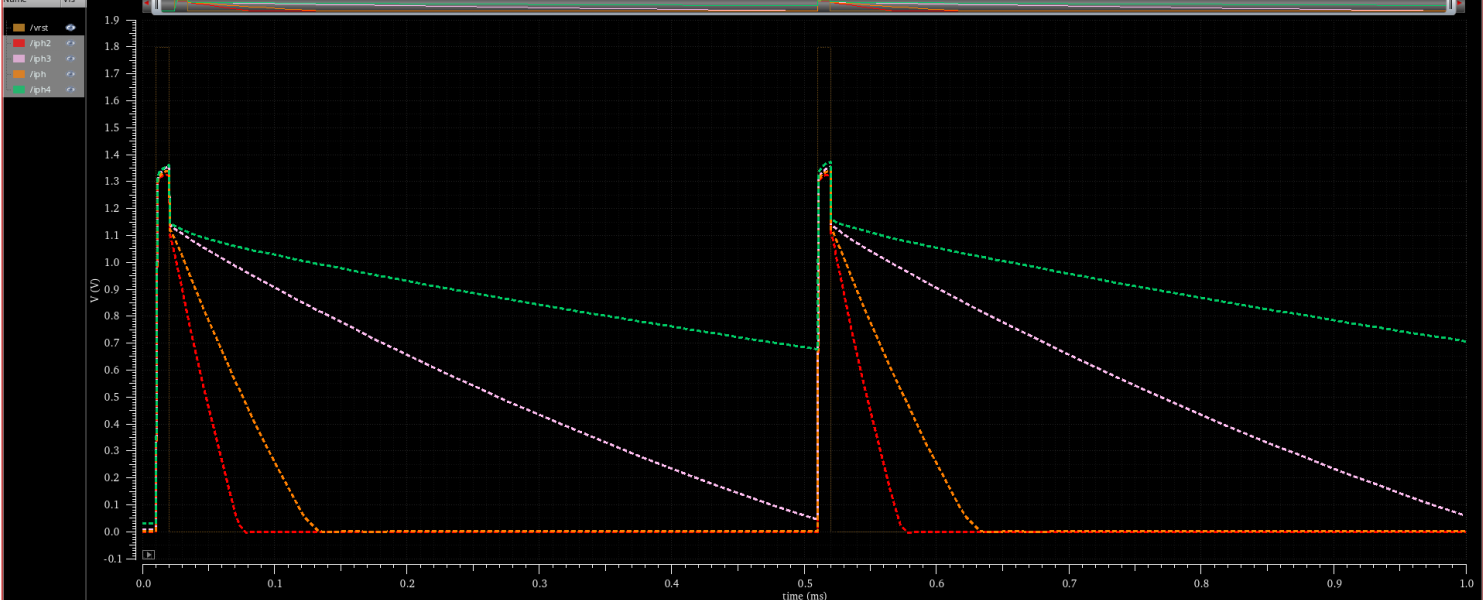
\includegraphics[height =0.2\textwidth]{differentslopes.png}
	\caption{Example charge decrease on 4 identical APS with photocurrents 1,10,20, and 50pA. For maximal range, inter-read time is dictacted by time needed for max current to deplete.}
	\label{differentslopes.png}
\end{figure}

\subsection{Column Readout}
\begin{figure}[h]
	\centering
	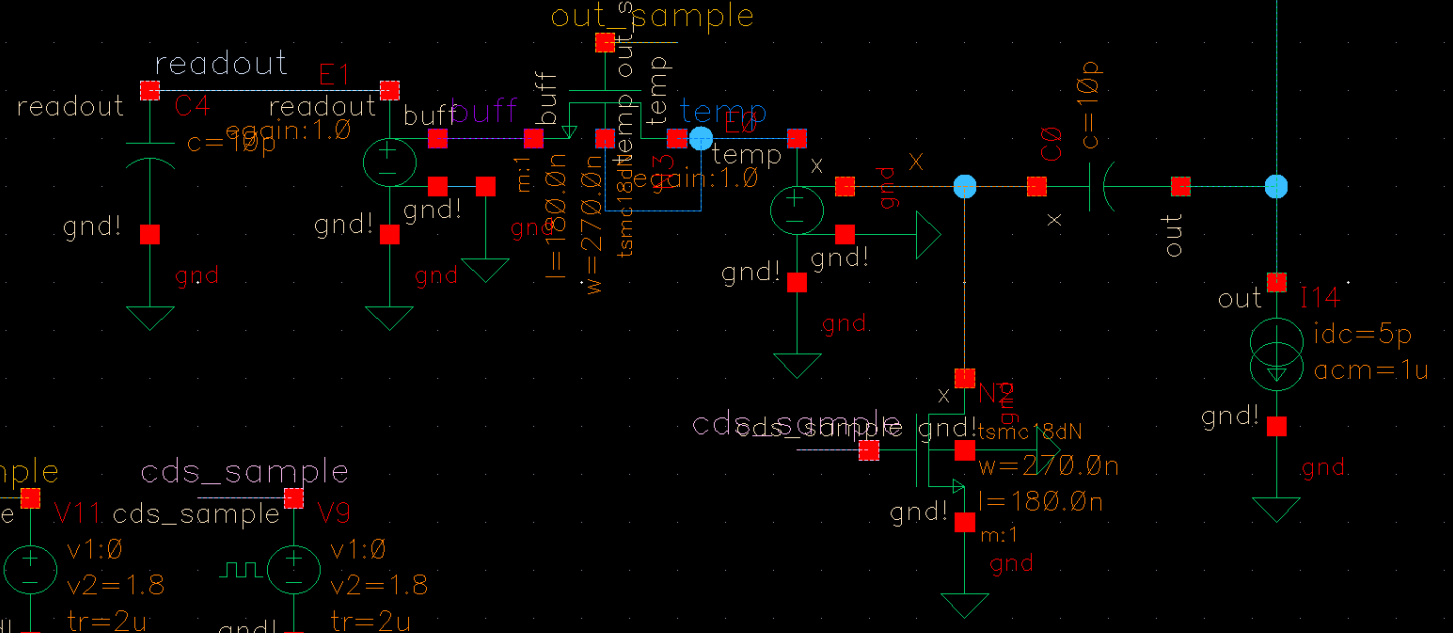
\includegraphics[width =0.3\textwidth]{readoutschem.png}
	\caption{Readout subcircuit}
	\label{readoutschem}
\end{figure}

The readout is organized as to read from an entire column at once, which is valid insofar as our select logic only chooses a single row of pixels at a time.
We need to have read each row within this timespan. While we could define our timing to evenly space the 4 rows in 160µs, we choose to read the row as quickly as possible (limited by a rise time of 500ns for all signals), and if necessary, wait until the next frame read becomes valid. 
We think this is more row-scaleable (there is additional space where the system 'reads' blank where more rows could easily be added) and could help to reduce motion blur, as the readout time between the first and Nth row is greatly reduced in this scheme.\\

The readout circuit consists of three parts: the capacitor connected on one side to the bus, is triggered by a switch, after which only the difference is propagated to the rest of the circuit. This difference then goes through a 'capturing' stage, again controlled by a signal out\_sample, which records a value at a given time for future reading. After this signal becomes low, future voltage values on the bus has no effect on the readout.
Finally, a tranmission gate is added to ensure that other readouts are left floating, unless asked to write to the output bus. Unless explicitly stated, the controlled input to this transmission gate is kept high for demonstration.
\subsection{C²MOS Select Logic}
\begin{figure}[h]
	\centering
	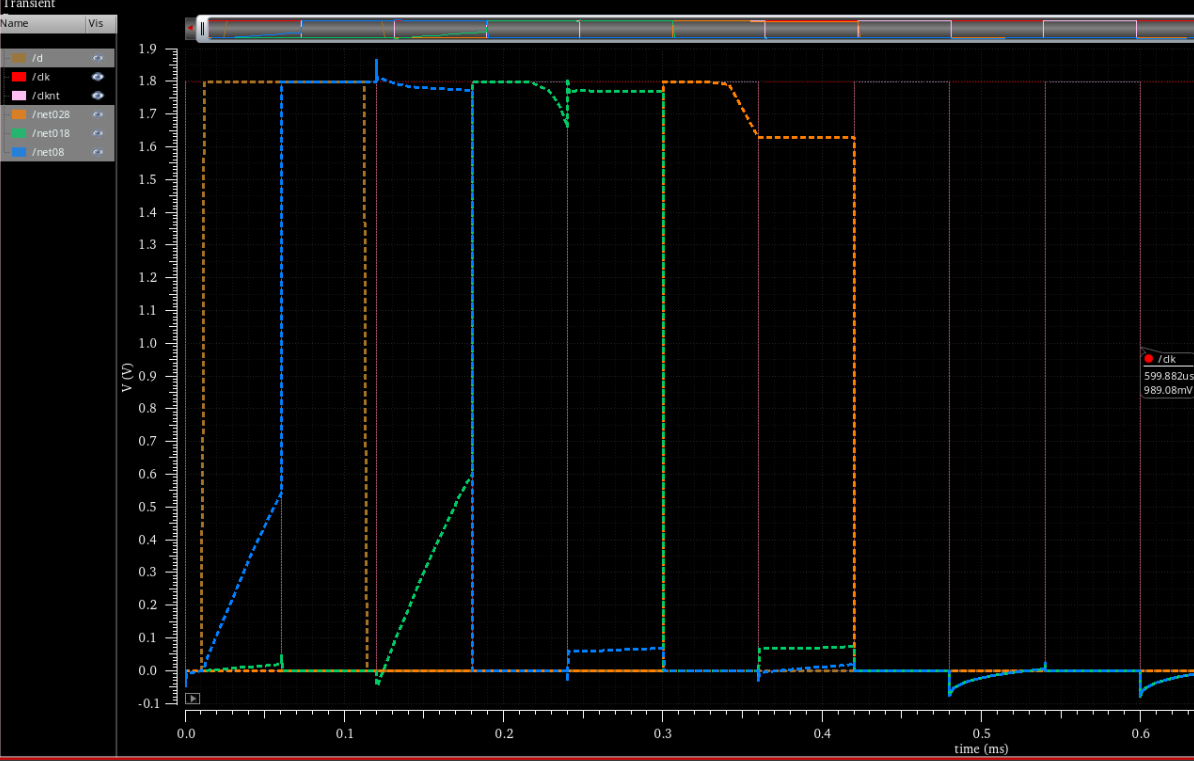
\includegraphics[width =0.3\textwidth]{shiftregisterpass.png}
	\caption{Shift register utilize one-hot encoding to connect a single row and column to the data and read buses  at any one time}
	\label{}
\end{figure}

We use a C²MOS implementation of a shift register to control the one-hot encoding of row select and column select.
This method is advantageous when compared to a classic shift register because it uses less transistors. It cannot store a bit in a static position indefinitely, but this design relies on the timing to be so fast that this is inconsequential.\\
\begin{figure}[h]
	\centering
	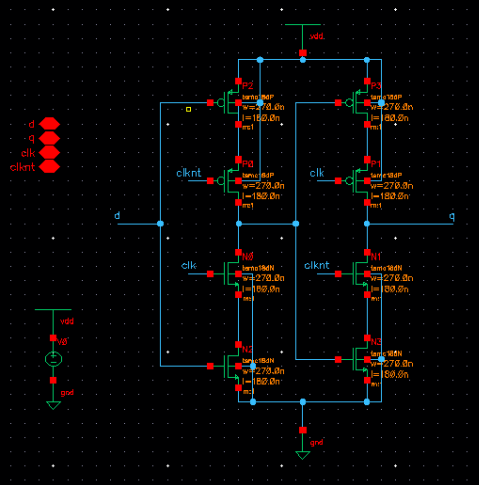
\includegraphics[width =0.3\textwidth]{c2mosschem}
	\caption{Single c²mos cell}
	\label{c2mosschem}
\end{figure}

We pitch-matched the C²MOS length (Figure \ref{shiftreglayout}) such that they stack directly on the APS columns and rows with no need for additional wiring. The clock and inverted clock signals are connected together, as are power signals and adjacent d-to-q input/outputs.
\begin{figure}[h]
	\centering
	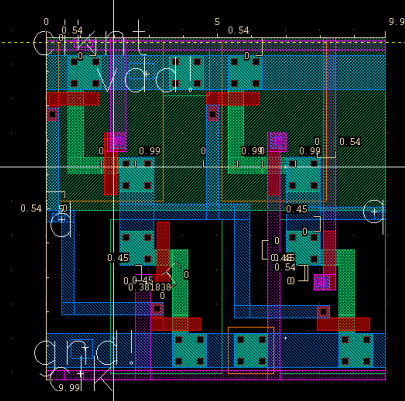
\includegraphics[width =0.3\textwidth]{shiftreglayout.png}
	\caption{Pitch-matched shift register layout}
	\label{shiftreglayout}
\end{figure}

Note the use of multiple pins to increase switching speed. This is particularly relevant for the readout bus registers, whose speed needs to increase with column count \cite{photodiodes}.
\subsection{Timing Protocol}
The local timing protocol of a pixel is straightforward: the row select decides which pixel in each column is allowed to communicate to the bus, during which time we send a dds\_sample signal, 
which 'captures' the voltage from the source follower (minus a $V_{DS}$ drop),
and is directly followed by a reset signal which puts the source follower voltage back to $V_{DD}-V_{DS\text{(cutoff)}}$.
The readout subcircuit copies the difference of the voltages seen during dds\_sample and v\_rst when out\_sample is pulsed high, which uncouples it from the voltage on the line and keeps it available until the row readout is ready to see it.
The readouts operate in parallel, after which the column C²MOS read sequentially in a single burst (Figure \ref{burstreadout}).
This way of reading pixel has the inherent advantage that the timing does not need to change when more rows and columns are added.
\begin{figure}[h]
	\centering
	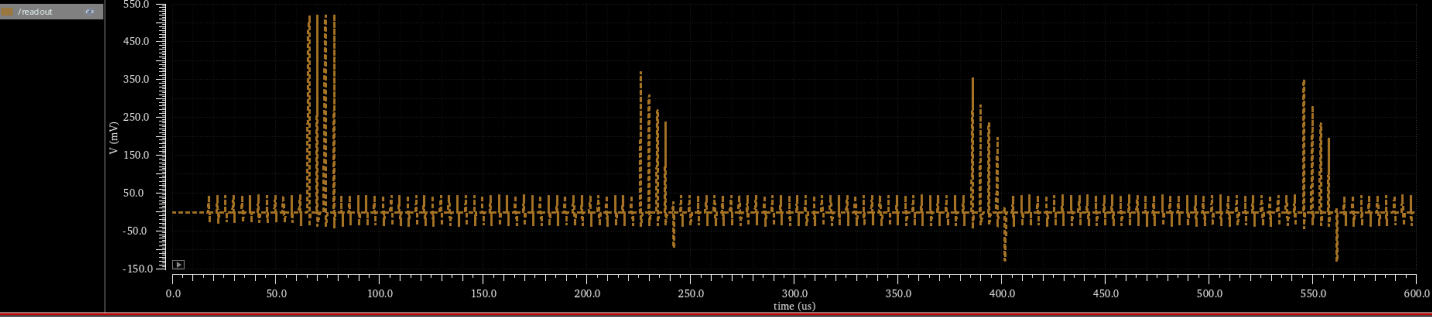
\includegraphics[width = 0.3\textwidth]{burstreadout.png}
	\caption{Example burst readout of 16 pixels}
	\label{burstreadout}
\end{figure}

\section{Experimental Results}

Figure \ref{exaggerated} emulates a changing environment by showing the readout of a single pixel with a varying current.
This is an over-dramatization of the phenomenon, but we find the voltage range under realistic conditions (1-4pA, adjusting for 'dark' current present even at no incoming brightness) to result in a much less appreciable variability.
This can be remedied with lower capacitor sizes in the source follower, but with minimal allowed sizes by the 180nm process we run into the practical issue that the percentage error in process size becomes significant, creating uneven sensibility between pixels in the frame.
To avoid this, we settle for a small voltage range and have a capacitor sized at 700nm, much larger than the theoretical minimum allowed size.
\begin{figure}[h]
	\centering
	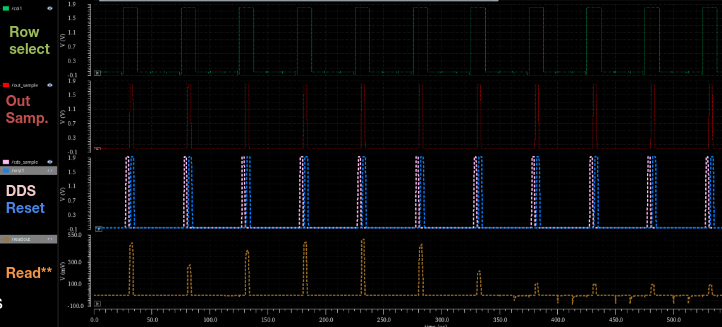
\includegraphics[width =0.3\textwidth]{exaggerated.png}
	\caption{Example results of single pixel with control signals timing, operating on a range of 0-200pA (exaggerated)}
	\label{exaggerated}
\end{figure}

\begin{figure}[h]
	\centering
	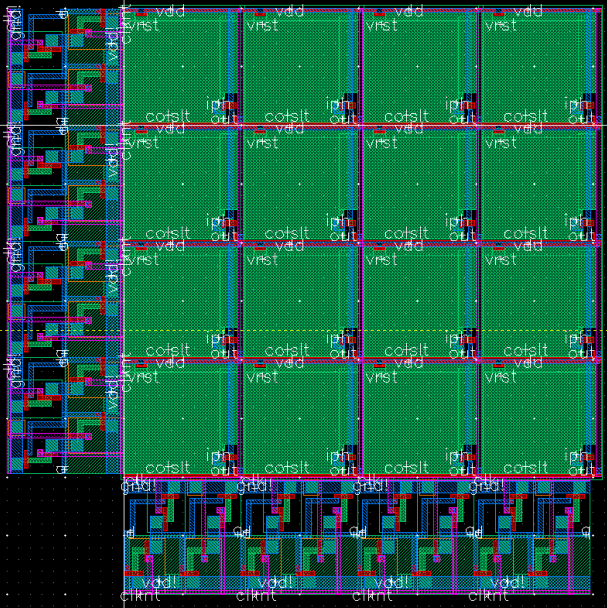
\includegraphics[width =0.3\textwidth]{fullarraylayout.png}
	\caption{Full 4 by 4 array configuration}
	\label{fullarrayreadout}
\end{figure}

\begin{figure}[h]
	\centering
	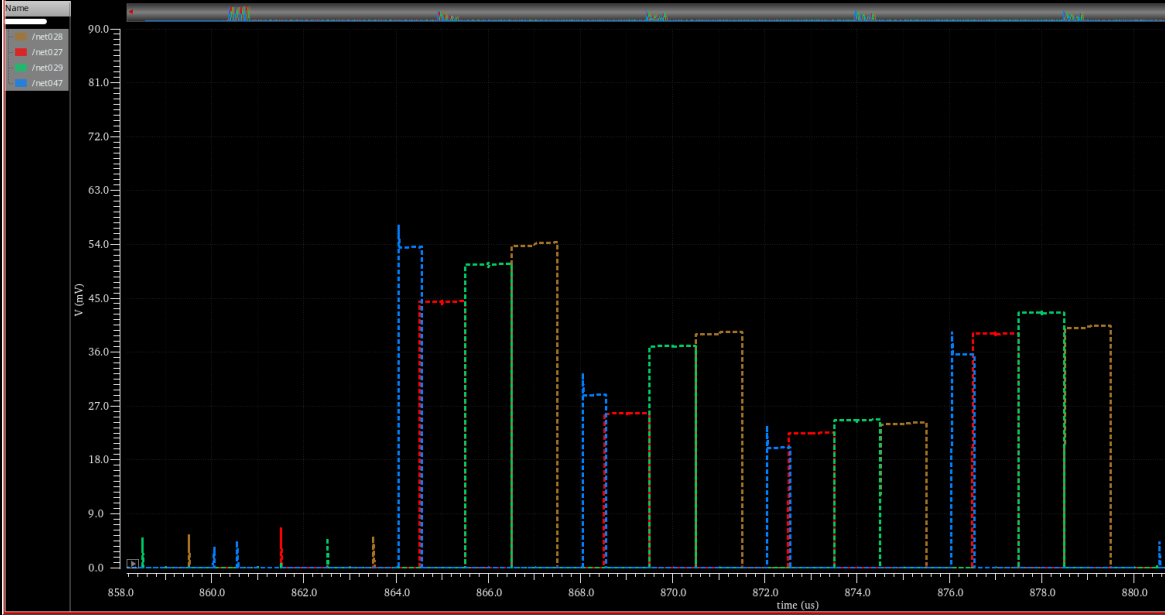
\includegraphics[width =0.3\textwidth]{fourcolreadoutBEST.png}
	\caption{Example readout of all 16 pixels}
	\label{fourcolreadout}
\end{figure}
\begin{figure}[h]
	\centering
	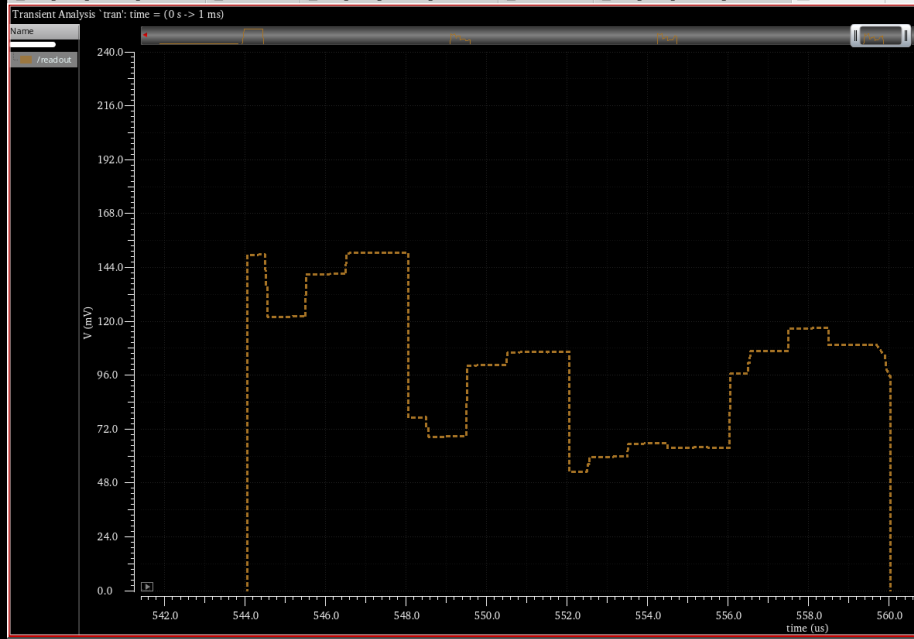
\includegraphics[width =0.3\textwidth]{transamelinereadout.png}
	\caption{Same as figure \ref{fourcolreadout}, with columns connected to the same line}
	\label{}
\end{figure}


\section{Discussion}
\subsection{Alternative Timing Protocols}
There are a variety of other potential timing schemes compatible with this architecture. A non-option is the most direct one, which is to reset a row of pixels and wait on that row for the required inter-reset period to complete.
This scheme is extremely slow, though it does remove the extra assumption of identical reset voltages on the source follower capacitor. Figure \ref{cmosyangwei} shows that this option is not viable for the C²MOS used here.
Another possible scheme is where the inter-reset interval is equally split into y intervals, where y is the amount of rows in the APS array.
This makes the timing much easier in that the output to the column shift register can double as the clock to therow shift register, but may lead to some "motion blur" across the rendered rows, since the first and Yth row read their data at very different intervals.
Note that in very large arrays where the minimum row read time is close to $\frac{t_{\text(inter-reset)}}{Y}$, this is essentially the same scheme as the one used here, with the added benefit of less timing logic.\\

Finally we revisit the importance of the out\_sample subcircuit used in this implementation. We see from Figure \ref{nooutsample} that not storing all the column readouts simultaneously, and instead reading them one at a time according to the column shift register, causes gradual dips in between readings, which is clearly not desired.
We note, however, that in some cases it may be advantageous to remedy this by having an additional shift register to sequentially activate the v\_reset signals along a row, rather than the current implementation; this one introduces yet another voltage drop along the out\_sample transistor because 
\begin{figure}[h]
	\centering
	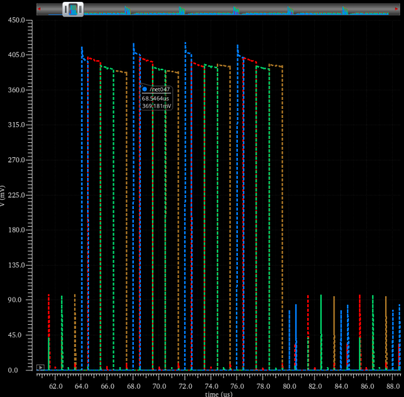
\includegraphics[width =0.3\textwidth]{nooutsample.png}
	\caption{Example readout with transparent readout output- (no storage with out\_sample)}
	\label{nooutsample}
\end{figure}

\subsection{Tiling Methodology}
Figure \ref{qdcontact} shows some of the techniques employed to allow for easy very large scale integration of the pixel array. Though gates need to be made of polysilicon, sections that have to cover long distances (particularly clock and control signals) are preferred as metals to increase switching speed.
\begin{figure}[h]
	\centering
	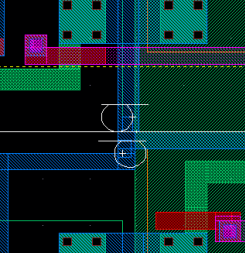
\includegraphics[width =0.3\textwidth]{qdcontact.png}
	\caption{Careful positioning of nets in shift register layout minimizes the external wiring needed for adapting the array to very large scale}
	\label{qdcontact}
\end{figure}


\begin{figure}[h]
	\centering
	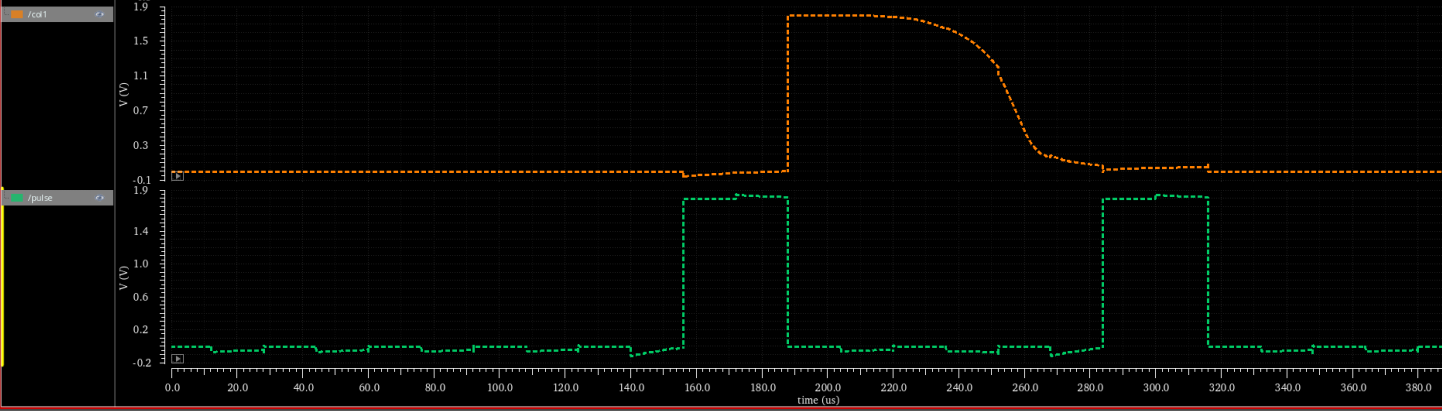
\includegraphics[width =0.3\textwidth]{cmosyangwei.png}
	\caption{C²MOS cannot hold charge for a significant amount of time}
	\label{cmosyangwei}
\end{figure}

\section{Conclusion}
As a final step, we scale up the pixel array to a full area of 2.5 by 2.5mm from its original 50 by 50 µm (Figure \ref{fullframe}). This is easily done as per the methods described in a previous section, where only edge-to-edge placement has to be considered.
In this paper we have tried to apply VLSI design principles and the device physics of photodiodes into a functional camera design.
\begin{figure}[h]
	\centering
	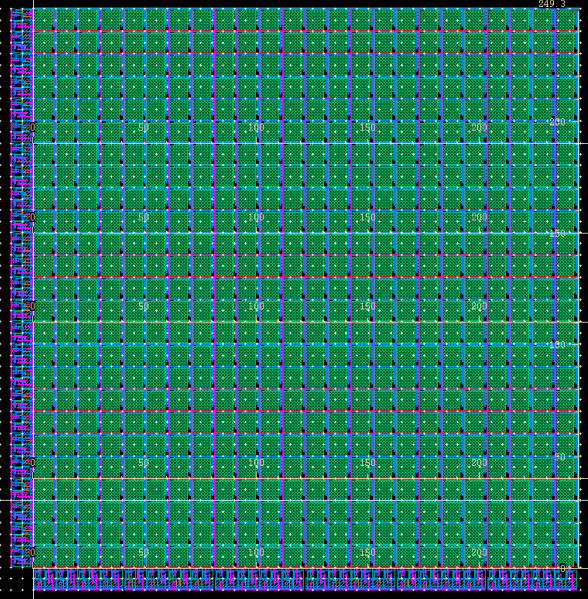
\includegraphics[width =0.3\textwidth]{fullframe.png}
	\caption{Full-sized 2.5mm pixel array}
	\label{fullframe}
\end{figure}

\section{Engineering Ethics}
	Due to the increasing affordability of CMOS processes, inexpensive electronics, and indeed camera equipment, have become ubiquitous in everyday electronics.
	The writers of this paper subscribe to the code of ethics stipulated by IEEE 7000-2021 standard with respect to formulating a clear mission statement aimed at elevating societal and ecological systems \cite{ieee7001}.
\printbibliography
\end{document}
